\documentclass[12pt,fleqn]{article}

\usepackage[utf8]{inputenc}
\usepackage[T2A]{fontenc}
\usepackage{amssymb,amsmath,mathrsfs,amsthm}
\usepackage[russian]{babel}
\usepackage[pdftex]{graphicx}

\usepackage[footnotesize]{caption2}
\usepackage{indentfirst}
\usepackage{bbm}
\usepackage{siunitx}
\usepackage{enumitem}
\usepackage[colorlinks, unicode]{hyperref}
%\usepackage[ruled,section]{algorithm}
%\usepackage[noend]{algorithmic}
%\usepackage[all]{xy}

% Параметры страницы
\textheight=24cm % высота текста
\textwidth=16cm % ширина текста
\oddsidemargin=0pt % отступ от левого края
\topmargin=-1.5cm % отступ от верхнего края
\parindent=24pt % абзацный отступ
\parskip=0pt % интервал между абзацам
\tolerance=2000 % терпимость к "жидким" строкам
\flushbottom % выравнивание высоты страниц
%\def\baselinestretch{1.5}
\setcounter{secnumdepth}{0}
\renewcommand{\baselinestretch}{1.1}

\newcommand{\norm}{\mathop{\rm norm}\limits}
\newcommand{\real}{\mathbb{R}}

\newcommand{\ex}{\mathbb{E}}
\newcommand{\diag}{\mathrm{diag}}
\newcommand{\intset}{\mathrm{int}}
\newcommand{\softmax}{\mathop{\rm softmax}\limits}
\newcommand{\lossfunc}{\mathcal{L}'}
\newcommand{\elbo}{\mathcal{L}}
\newcommand{\normal}[3]{\mathcal{N}(#1 | #2, #3)}
\newcommand{\dd}[2]{\frac{\partial#1}{\partial#2}}
\newcommand{\kl}[2]{\mathop{KL}(#1 \parallel #2)}
\newcommand{\nm}{\mathcal{N}}
\newcommand{\sle}{\; \Rightarrow \;}
\newcommand{\indpos}{\mathbf{I}_{d_k}^{+}[i, j]}
\newcommand{\indneg}{\mathbf{I}_{d_k}^{-}[i, j]}

\usepackage{pgfplots}
\graphicspath{ {./images/} }
\begin{document}

\begin{titlepage}
    \begin{center}
	{\small \sc Московский государственный университет \\имени М.~В.~Ломоносова\\
	Факультет вычислительной математики и кибернетики\\}
	\vfill
	{\large \bf\MakeUppercase{Композиции алгоритмов для решения задачи регрессии} }\\ 
	~\\
	{\large \bf ЗАДАНИЕ №3}
	~\\
	~\\
	~\\
	~\\
	{\large \sc Практикум 317 группы}\\ 
	~\\
	{\large \bf ОТЧЕТ}\\ 
	{\large \bf о выполненном задании}\\
	{\large \br студента 317 учебной группы факультета ВМК МГУ}\\
	{\large \br Кузнецова Михаила Константиновича}\\
    \end{center}
    \begin{center}
	\vfill
	{\small Москва\\2020}
    \end{center}
\end{titlepage}

\section{Введение}
В данной работе рассматривается применение методов случайных лес и градиентный бустинг для задачи определения стоимости жилья. Исследуется влияние различных гиперпараметров на поведение моделей.

\section{Эксперименты}
\subsection{Начальная обработка данных}
Проведены следующие трансформации датасета:

\begin{enumerate}[noitemsep]
    \item удаление столбцов <<index>>, <<id>>, <<date>> из матрицы признаков
    \item удаление столбца <<index>> из признаков целевого датасета
\end{enumerate}

\subsection{Влияние гиперпараметров}
Исследуем поведение случайного леса и градиентный бустинга для задачи регрессии в зависимости от \emph{n\_estimators}, \emph{feature\_subsample\_size}, \emph{max\_depth} и \emph{learning\_rate} для градиентного бустинга. Выбраны следующие дефолтные значения:

\begin{center}
\begin{tabular}{|c|c|c|}
\hline parameter & rf & boosting  \\
\hline n\_estimators & 75 & 75 \\
\hline feature\_subsample\_size & None & None \\
\hline max\_depth & None & 5 \\
\hline learning\_rate & -- & 0.1 \\
\hline
\end{tabular}
\captionof{table}{Значения по умолчанию моделей}
\end{center}

\subsubsection{\emph{n\_estimators}}
\begin{figure}[h]
    \centering
    \subfigure{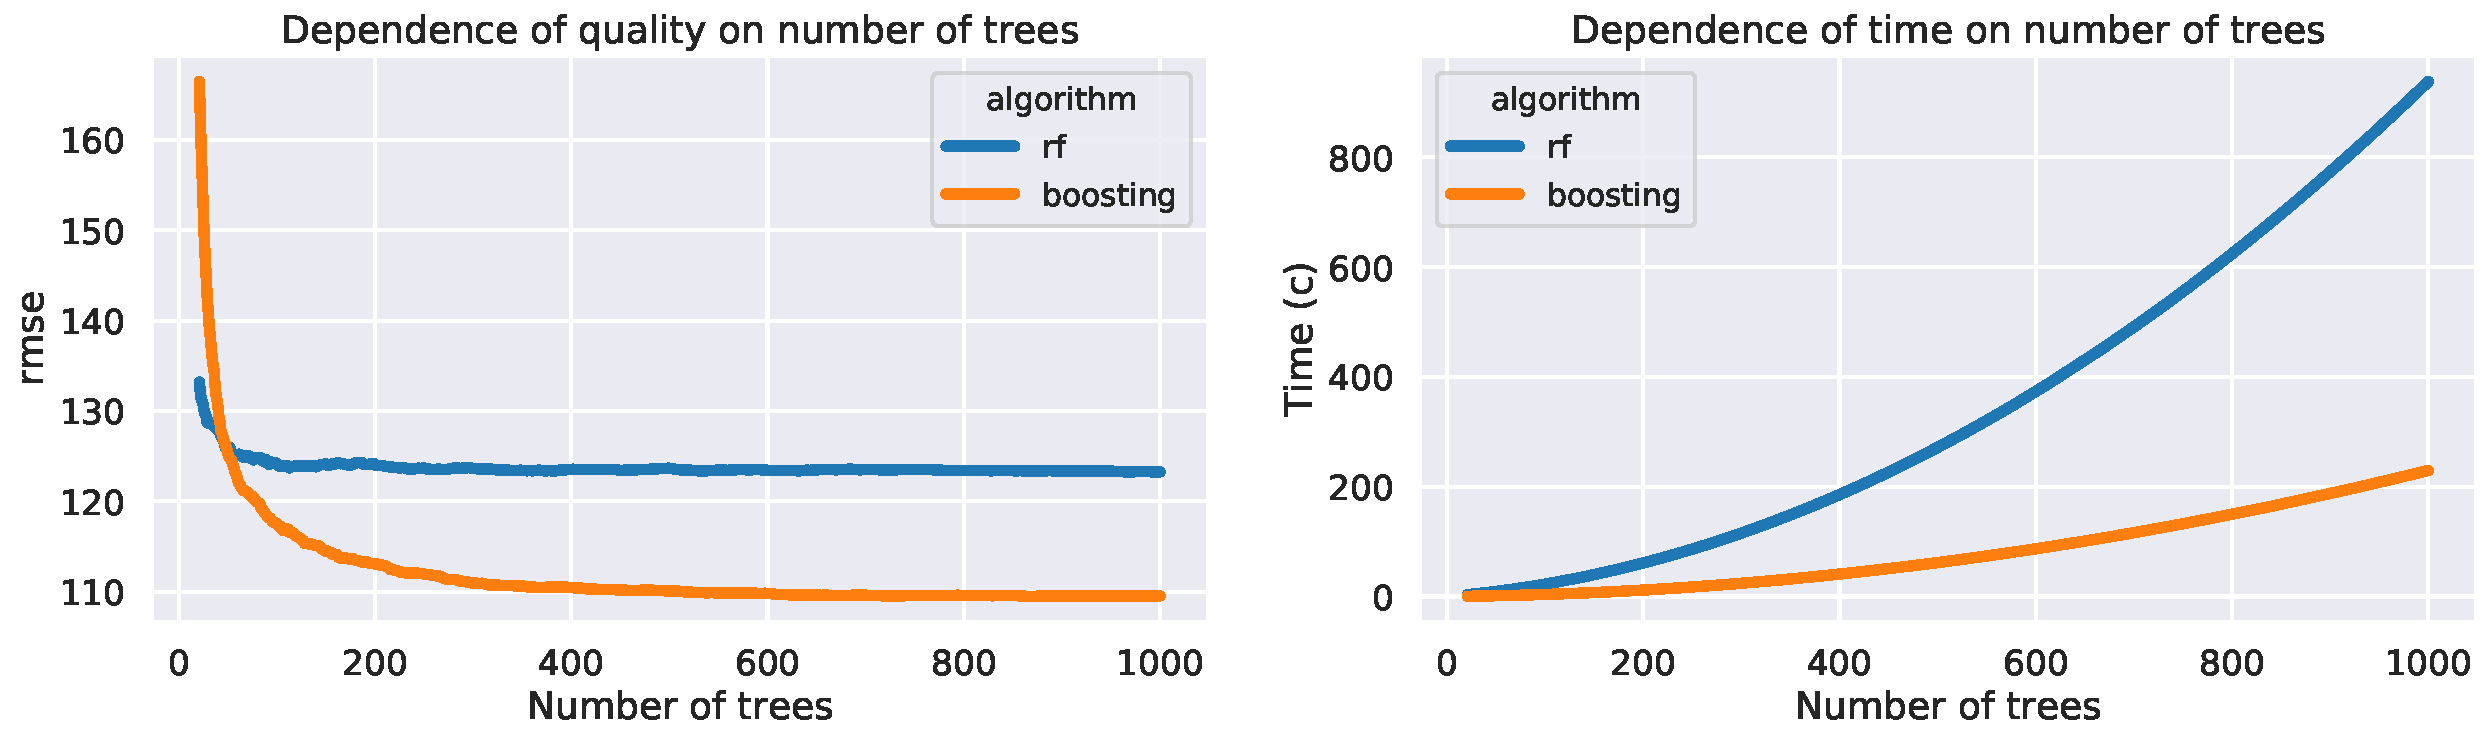
\includegraphics[width=0.99\textwidth]{all/3/images/n_estimators.pdf}}
\end{figure}
Качество постепенно растёт с увеличением количества деревьев в boosting методе, а в rf достигает максимума при 75 деревьев. Причиной этому может стать разница в значении \emph{max\_depth}. Заметим, что время обучения зависит приблизительно линейно от количества деревьев. 
\newpage

\subsubsection{\emph{feature\_subsample\_size}}
\begin{figure}[h]
    \centering
    \subfigure{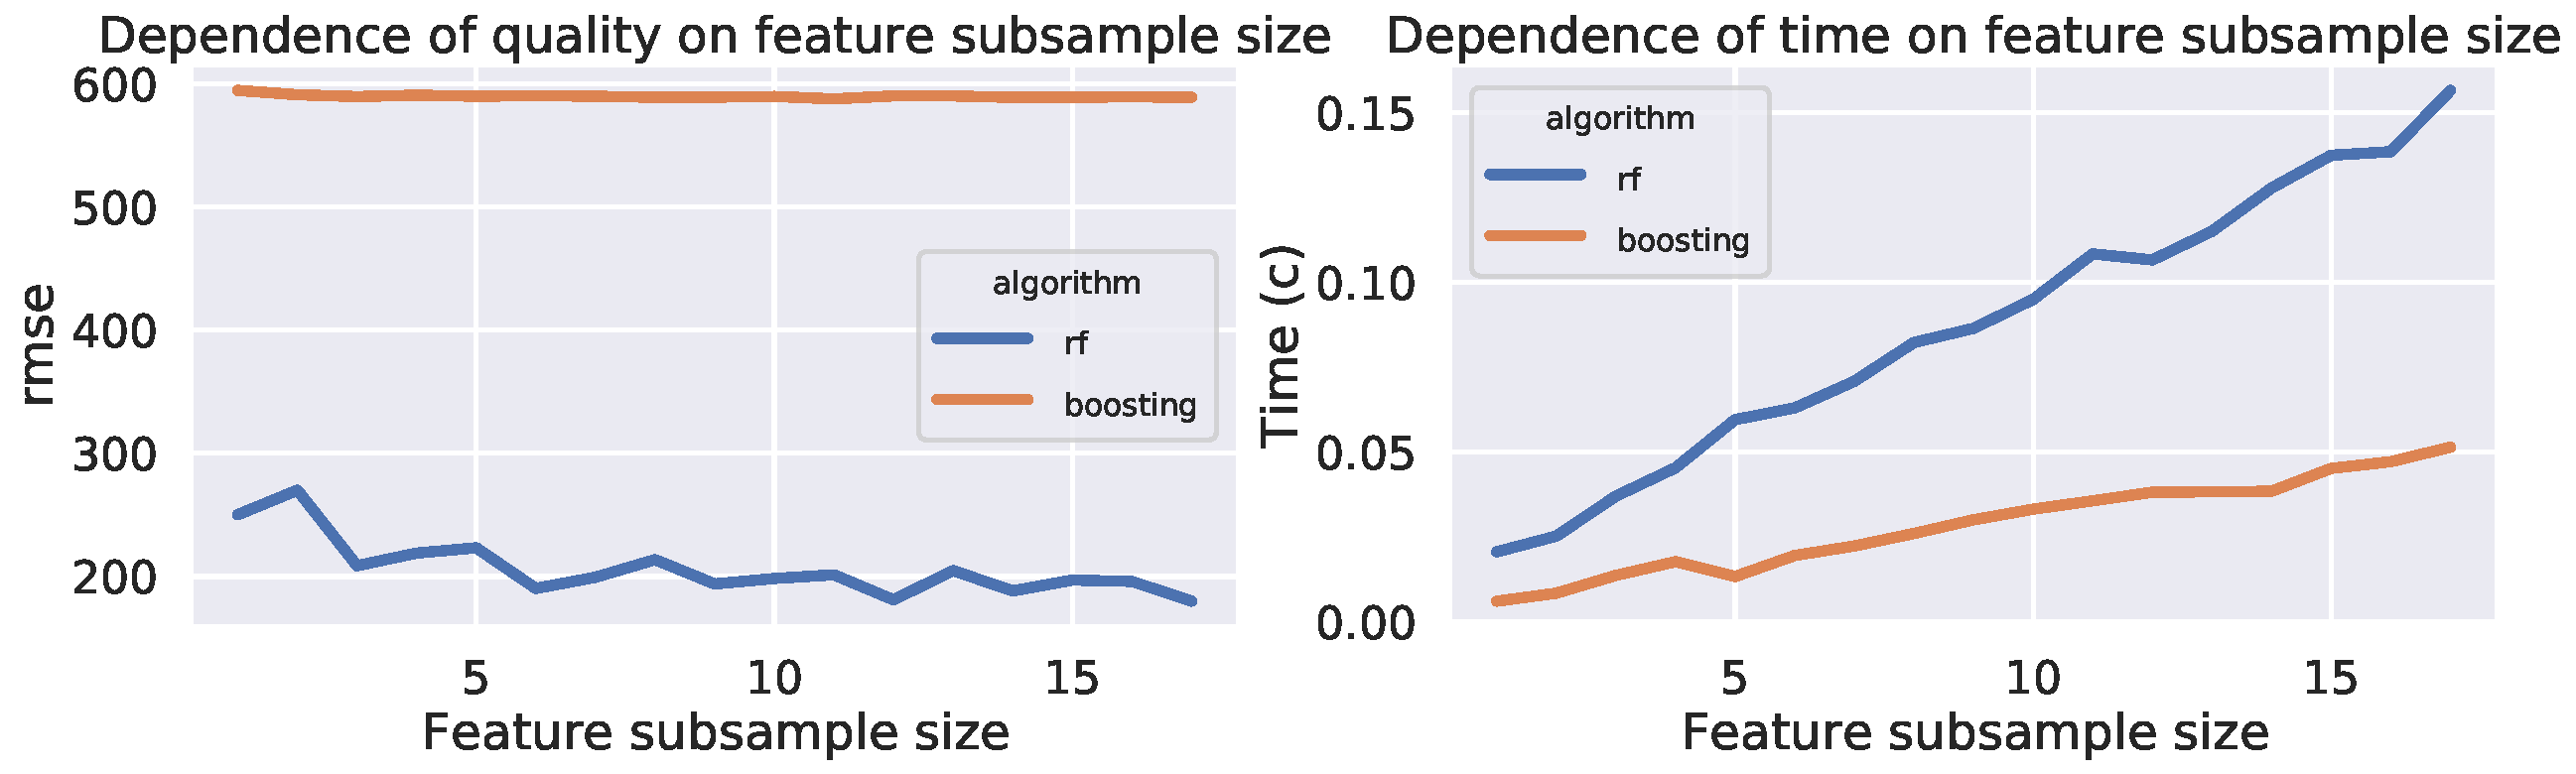
\includegraphics[width=0.99\textwidth]{all/3/images/feature_subsample_size_gen.pdf}}
\end{figure}

Наблюдается логичное улучшение качества при увеличении данного параметра. Линейная зависимость времени позволяет удобно подобрать параметр в определенных условиях задачи. Так как \emph{max\_depth} = None в rf, большой данный параметр не поможет построить различные деревья. В случае с boosting глубина не велика. Это даёт возможность постепенного увеличения качества.

\subsubsection{\emph{max\_depth}}
\begin{figure}[h]
    \centering
    \subfigure{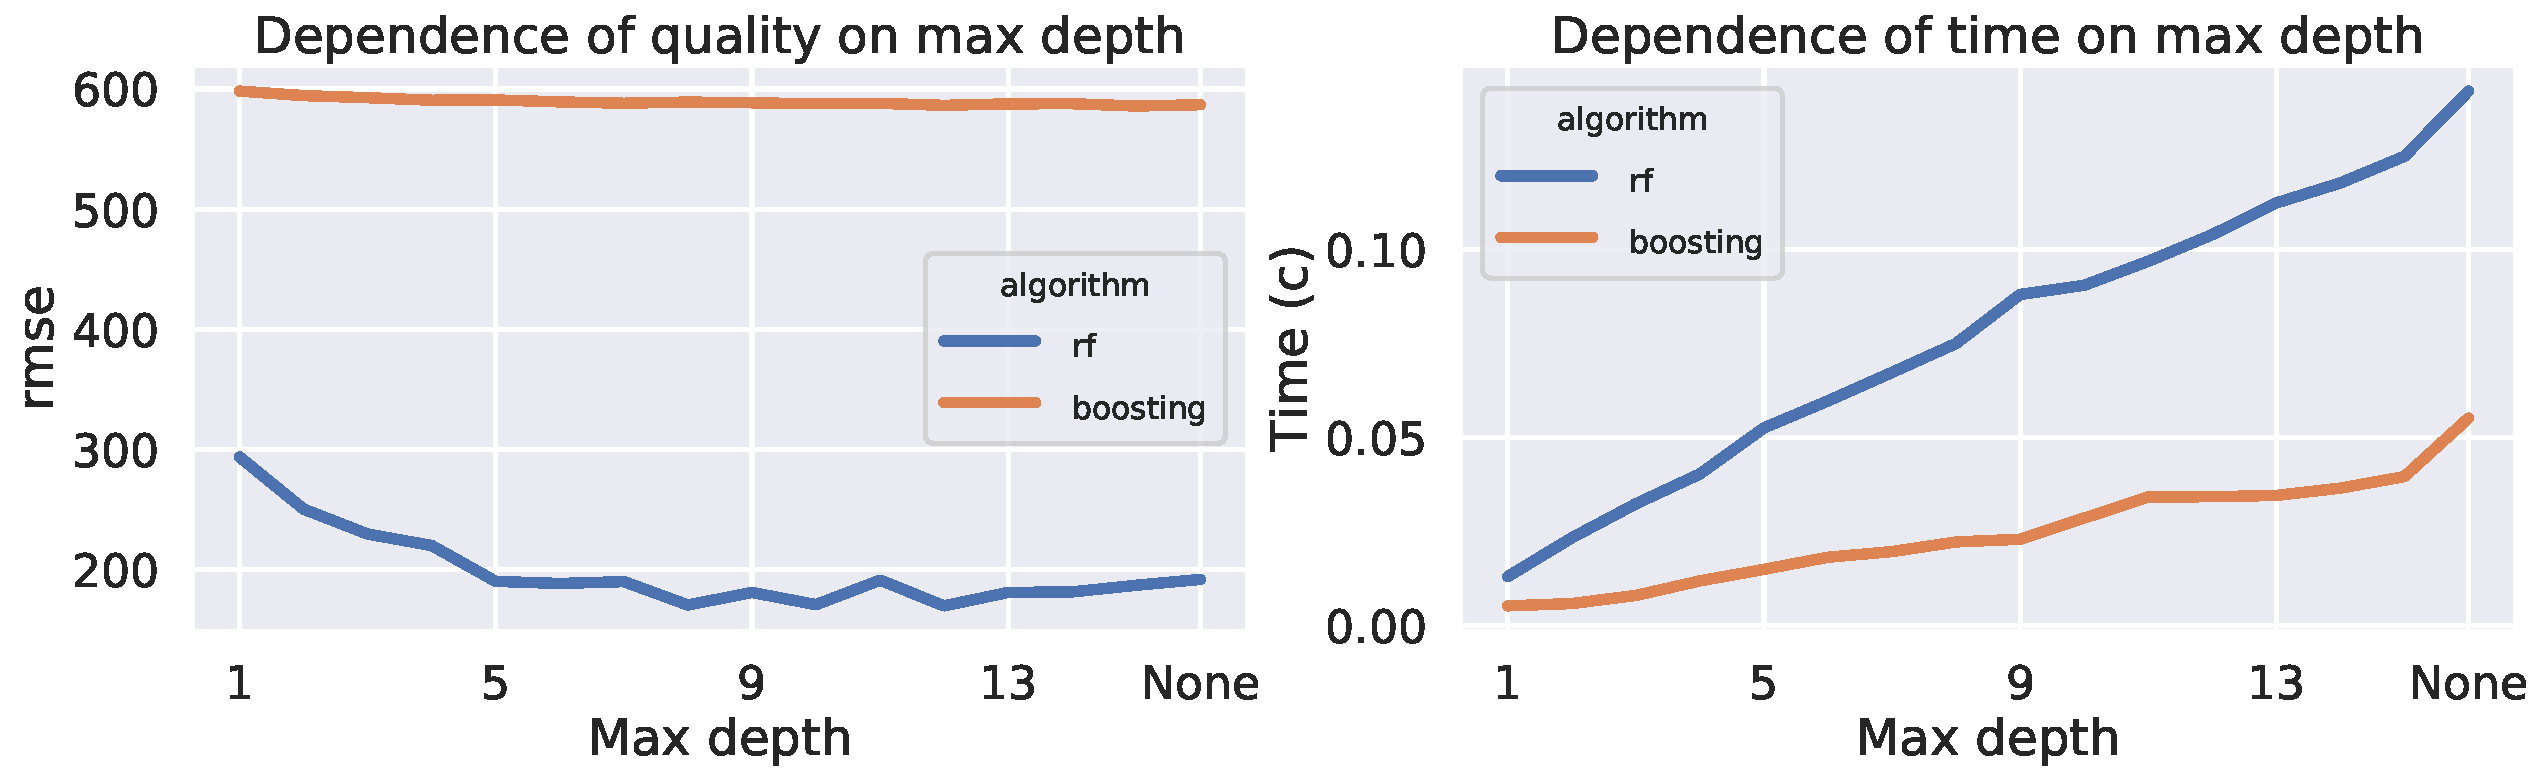
\includegraphics[width=0.99\textwidth]{all/3/images/max_depth_gen.pdf}}
\end{figure}

Отчётливо видно, что boosting над слишком простыми или сложными моделями даёт плохое качество. Есть линейная зависимость между временем и глубиной дерева. 
\newpage

\subsubsection{\emph{learning\_rate}}
\begin{figure}[h]
    \centering
    \subfigure{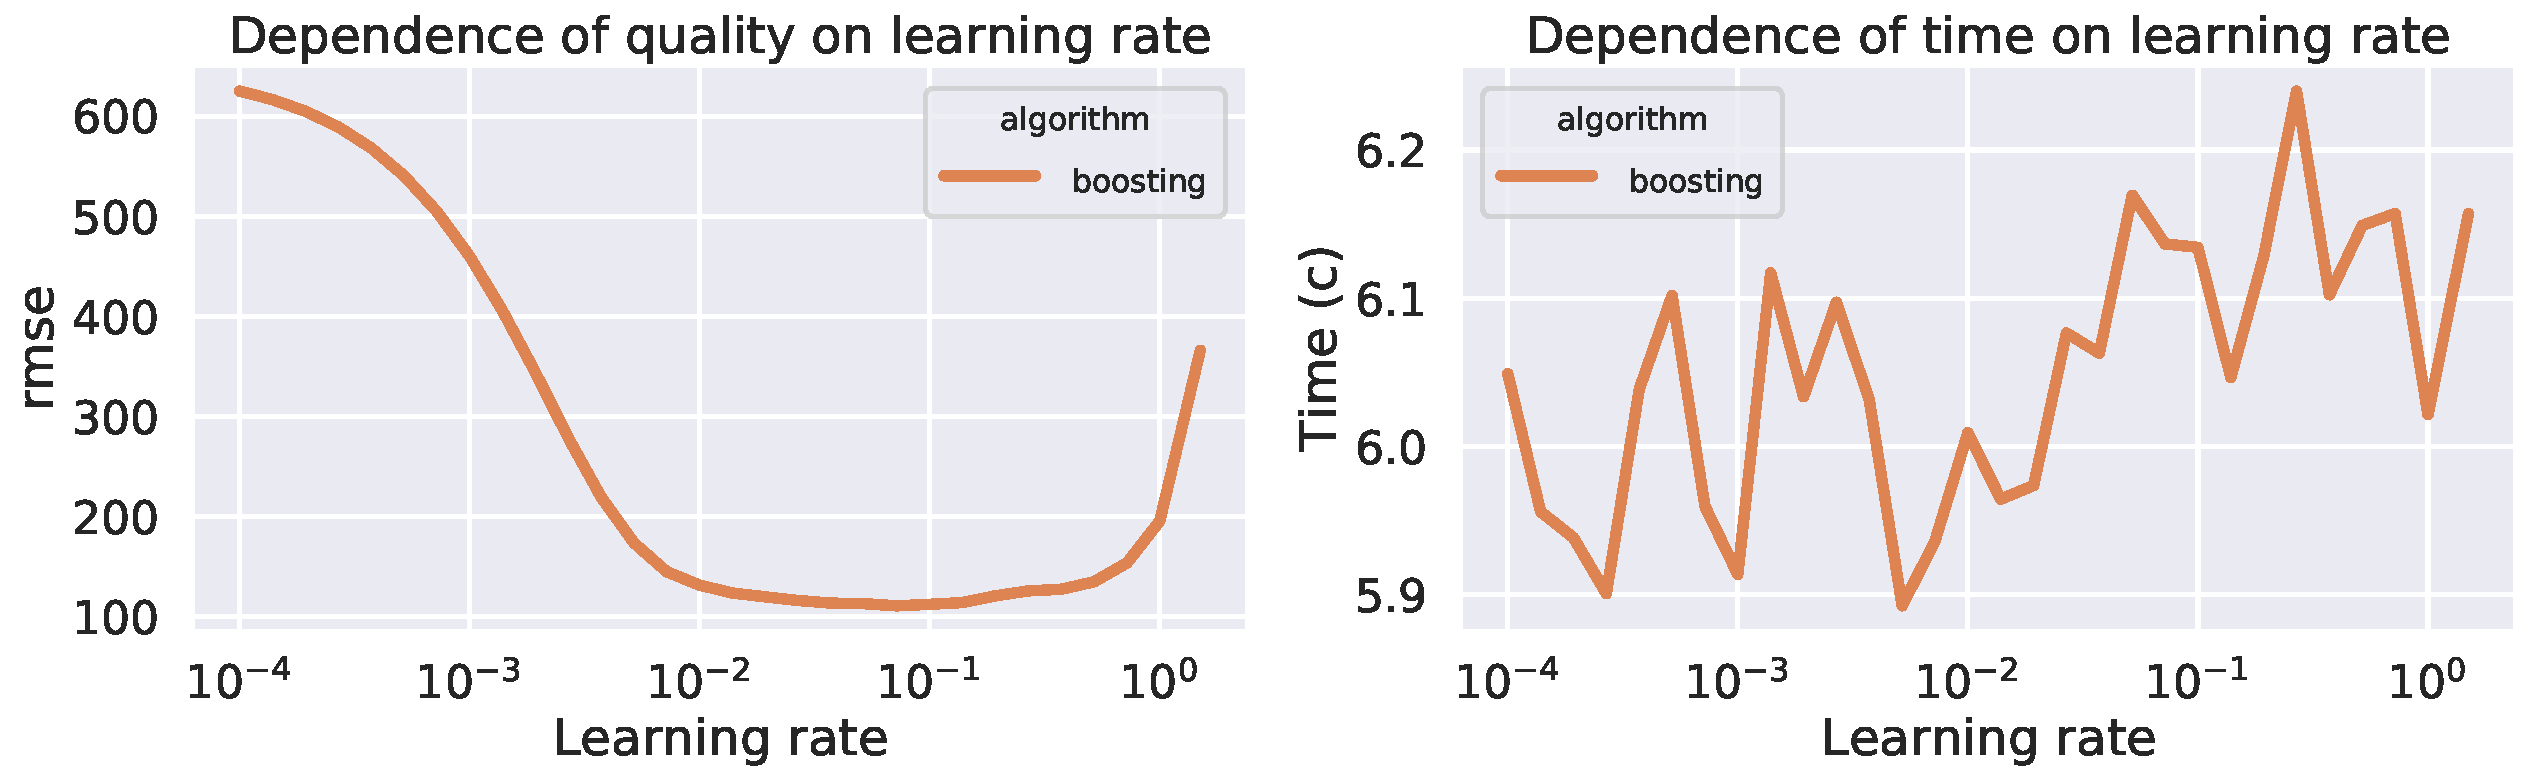
\includegraphics[width=0.99\textwidth]{all/3/images/learning_rate.pdf}}
\end{figure}

Маленький \emph{learning\_rate} --- не доходим до оптимума, большой --- перескакиваем его. Аналогично с временем: маленький --- слабо сдвигаем ошибки предыдущих ответов, следовательно, последующие модели будут сталкиваться с теми же проблемами, большой --- приводит к исправлениям ответов с неправильным мультипликатором. 


\section{Выводы}
В работе представлены экспериментальные результаты, касающиеся задачи регрессии для случайного леса и градиентного бустинга. Проведена сравнительная характеристика. В условиях данного эксперимента можно выделить следующие тезисы:
\begin{itemize}[noitemsep]
    \item при увеличении количества деревьев, с какого то момента rf не улучшает качество, а boosting наоборот
    \item $~\frac{number\ of\ features}{2}$ является оптимальным \emph{feature\_subsample\_size} для rf
    \item для обоих алгоритмов небольшая глубина является оптимальной 
    \item \emph{learning\_rate} имеет большое значение на сходимость метода  
\end{itemize}

\end{document}
